\documentclass{article}
\usepackage[UTF8]{ctex}
\usepackage{amsfonts}
\usepackage{amsmath}
\usepackage{float}
\usepackage{graphicx}
\usepackage{color}

% paragraph
\setlength{\parindent}{0pt}
\setlength\parskip{\baselineskip}
\renewcommand{\baselinestretch}{1.2}

\begin{document}

% 标题
\title{《计算机辅助几何设计》作业}
\author{ID号: 46  \qquad  姓名: 刘紫檀}  %递交作业时填上ID号和姓名
\date{\today}
\maketitle

1. 证明:以下曲线是平面曲线,
$$
c(t) = (\frac{1 + t^2}{t}, t + 1, \frac{1-t}{t})
$$

只要计算密切平面的法向量即可。
\begin{align*}
c'(t) &= (1 - \frac{1}{t^2}, 1, -\frac{1}{t^2}) \\
c''(t) &= (\frac{2}{t^3}, 0, \frac{2}{t^3})
\end{align*}
法向量为 $ \alpha(t) = c'(t) \times c''(t) / (\|c'(t)\| \|c''(t)\|) $,我们有
\begin{align*}
	\|c'(t)\| \|c''(t)\| \alpha(t)
	&= c'(t) \times c''(t) \\
	&= \left| \begin{matrix}
		\vec{i} & \vec{j} & \vec{k} \\
		1-t^{-2} & 1 & -t^{-2} \\
		2t^{-3} & 0 & 2t^{-3} \\
	\end{matrix} \right|\\
	&= (2t^{-3}, -2t^{-3}, -2t^{-3})
\end{align*}
容易看出,法向量是不随 $ t $ 的改变而改变的。所以,所有的 $ t $ 共享同一个密切平面,则曲线为平面曲线。

2. 当半径为 $r$ 的“动圆”沿着半径为 $R$ 的“定圆”的外侧无滑动地滚动时,动圆圆周上的一定点 $p$ 所描绘的点的轨迹,叫做外摆线。计算外摆线的参数曲线,并画出当 $r = 1, R = 3$ 时的曲线形状。

% 全网热议的“硬币悖论”怎么算?直觉为何欺骗了我们?
% https://www.bilibili.com/video/BV1Lb4y1X7cX/
% https://www.youtube.com/watch?v=vI2sSldLQr8

首先建立两个参考系 $ C_R $ 和 $ C_r $,如图所示
\begin{figure}[H]
	\centering
	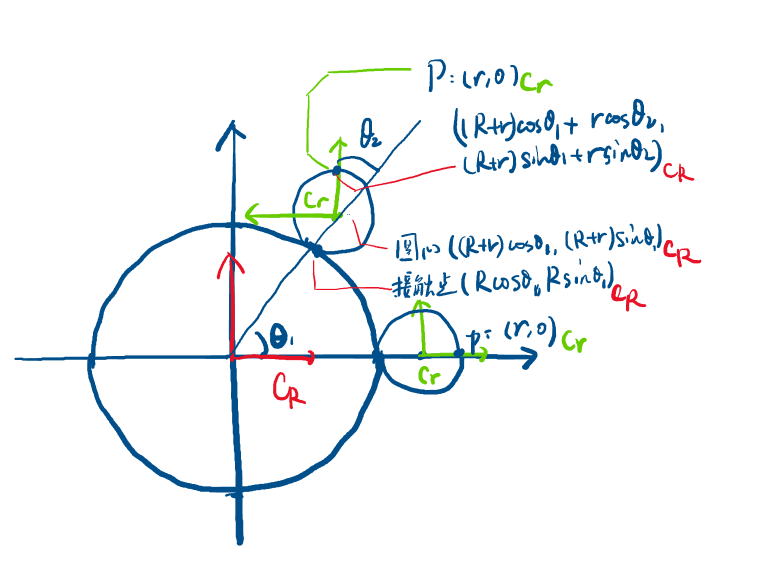
\includegraphics[width=\textwidth]{fig-1}\\
	\label{fig:fig-1}
\end{figure}
下面要找出 $ \theta_1 $ 和 $ \theta_2 $ 的关系。我们知道,所谓纯滚动,就是两圆的接触点在接触时没有相对运动。

为了方便,设小圆绕大圆滚动,则 $ C_r $ 相对 $ C_R $ 有 $ \vec{w_r} $ 的转动,$ \vec{v_r} $ 的平动。小圆与大圆的接触点相对 $ C_r $ 静止,其相对 $ C_R $ 的速度为 $ \vec{w_r} $ 和 $ \vec{v_r} $ 的合成,即 $ \vec{w_r} \times \vec{r} + \vec{v_r} $,同时和其接触的大圆与小圆的接触点的速度在 $ C_R $ 中为 0,则有
$$
\vec{w_r} \times \vec{r} + \vec{v_r} = 0
$$
成立。
我们知道,滚动时,$ v_r $ 一定平行于大圆的切线,否则之后两圆将分离或相交。这样,情形就只有下图所示的一种了:
\begin{figure}[H]
	\centering
	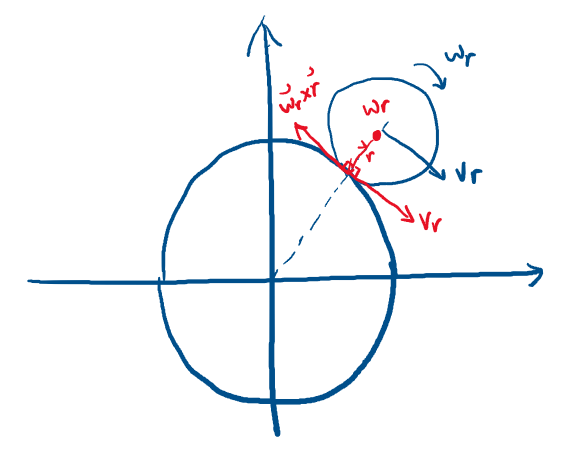
\includegraphics[width=0.8\textwidth]{fig-2}\\
	\label{fig:fig-2}
\end{figure}

那么,我们就可以得到 $ w_r r = v_r $(此处不带矢量符号表示模长),也就是说
\begin{align*}
	(R+r)\frac{\partial \theta_1}{\partial t} &= r \frac{\partial \theta_2}{\partial t}\\
	\theta_1 &= \theta_2 \frac{r}{R+r} \quad \text{(两边积分)}
\end{align*}

设 $ \theta = \theta_1 $,得到参数曲线如下:
\[
\begin{cases}
	x(\theta) = (R+r) \cos \theta + r \cos (R \theta / r + \theta) \\
	y(\theta) = (R+r) \sin \theta + r \sin (R \theta / r + \theta)
\end{cases}
\]
$ R = 3, r = 1 $ 时曲线形状如下(蓝色为曲线,红色和黄色分别为大圆和小圆):
\begin{figure}[H]
	\centering
	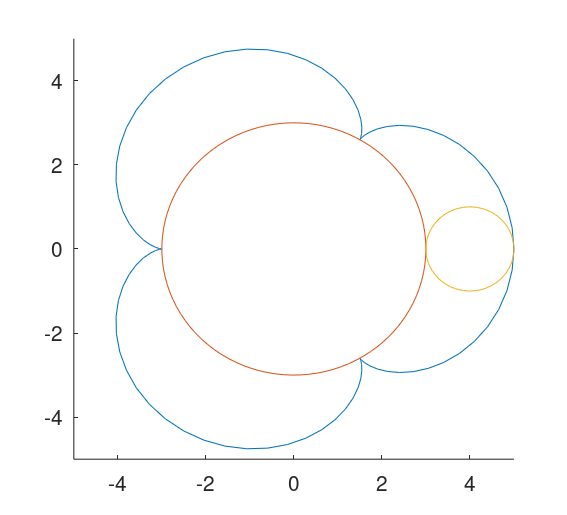
\includegraphics[width=0.6\textwidth]{fig-3}\\
	\label{fig:fig-3}
\end{figure}

3. 渐屈线是曲线上密切圆圆心的轨迹。特别的,Frenet 标架为 $ \{e_1(t), e_2(t)\} $ 的平面 Frenet 曲线 $ c : D \rightarrow \mathbb R ^2 $ 的渐屈线可由以下参数曲线 $ \eta : D \rightarrow \mathbb R^2 $ 表示,
$$
\eta(t) = c(t) + \frac{1}{\kappa(t)} e_2(t)
$$
编写程序画出椭圆的渐屈线及下图中标记点的密切圆(图略)。

首先由椭圆的参数方程计算椭圆的 Frenet 标架表示:
\begin{align*}
	e_1(t) &= \frac{c'(t)}{\|c'(t)\|} = (-\frac{a \sin t}{\|c'(t)\|}, \frac{b \cos t}{\|c'(t)\|})\\
	e_2(t) &= R^{90\deg} e_1(t) = (-\frac{b \cos t}{\|c'(t)\|}, -\frac{a \sin t}{\|c'(t)\|})
\end{align*}
计算曲率
% (-a*sin(t)/sqrt(a^2*sin(t)^2+b^2*cos(t)^2))'
$$
\kappa(t) = \frac{c'(t) \times c''(t)}{\|c'(t)\|^3} = \frac{ab}{(\sqrt{a^2 \sin^2t + b^2 \cos^2t})^3}
$$
则有
$$
\eta(t) = (a \cos t, b \sin t) + \frac{a^2 \sin^2t + b^2 \cos^2t}{ab} (-b \cos t, -a \sin t)
$$
那么在 $ c(t) $ 处的密切圆的圆心为 $ \eta(t) $,半径为 $ 1/{\kappa(t)} $ 。

下面的图展示了 $ a = 3, b = 1 $ 的椭圆,其渐屈线和 $ t $ 在 $ \pi/2, \pi, 11\pi/6 $ 时的密切圆。
\begin{figure}[H]
	\centering
	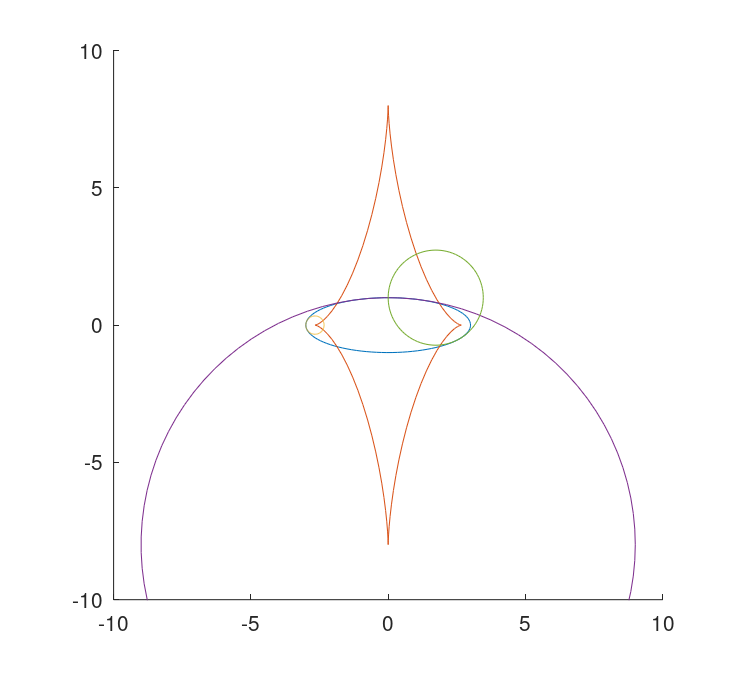
\includegraphics[width=\textwidth]{fig-4}\\
	\label{fig:fig-4}
\end{figure}
\end{document}
